% Capitulo 3

\chapter{Marco Teórico} % Main chapter title

\label{MarcoTeorico} % For referencing the chapter elsewhere, use \ref{Chapter1} 

\lhead{Capítulo 3 \emph{Marco Teórico}} % This is for the header on each page - perhaps a shortened title

%----------------------------------------------------------------------------------------

En este capítulo se introducen los conceptos necesarios que son indispensables conocer para el desarrollo del proyecto. Se considera como necesario todo aquel conocimiento que intervenga en el proceso de construcción del sistema y que sea crítico para el cumplimiento de los objetivos establecidos.

%----------------------------------------------------------------------------------------

\section{Aplicación Móvil}

Una aplicación móvil, más comúnmente conocida como una aplicación, es un tipo de software de aplicación diseñado para ejecutarse en un dispositivo móvil, como un ordenador smartphone o tablet. Las aplicaciones móviles sirven con frecuencia para proporcionar a los usuarios servicios similares a los que se accede en las PC. \cite{queParaApps}

Las aplicaciones móviles están diseñadas con la consideración de las exigencias y limitaciones de los dispositivos y también para aprovechar las capacidades especializadas que tienen.

Cabe mencionar que existen 3 tipos de aplicaciones móviles, las cuales pueden ser: 

\begin{itemize}
	\item \textbf{Nativas: }Diseñadas para exclusivamente correr en un sistema operativo específico.
	\item \textbf{Web: }Estas corren por medio de los navegadores propios de cada teléfono y  están configuradas para que puedan verse en un dispositivo móvil.
	\item \textbf{Híbridas: }Este tipo de aplicaciones resultan de la combinación de la anteriores como por ejemplo Facebook  que se descarga como una aplicación nativa pero se tiene que estar actualizando constantemente y que además puede verse de manera web en caso de no tener la aplicación instalada.\cite{tiposApps}
\end{itemize}

\section{Cómputo Móvil}

Sistema de computación en donde el usuario puede estar en movimiento, esto consiste en fabricar computadoras suficientemente pequeñas para ser fácilmente transportadas. Se tiene la necesidad de reemplazar los cables de conexión por una tecnología inalámbrica.

Este tipo de tecnología no solo representa una oportunidad de avance científico o computacional sino de implementar nuevas posibilidades de negocios como:

\begin{itemize}
	\item Aplicaciones financieras
	\item Gerencia de inventario
	\item Gerencias de servicios de campo
	\item Localización de productos
\end{itemize}

\subsection{Características de la Computación Móvil}

\begin{itemize}
	\item \textbf{Movilidad: }Implica la portabilidad basada en el hecho de que los usuarios llevan un dispositivo móvil a todas las partes a donde se dirigen, por lo tanto, los usuarios pueden iniciar el contacto en tiempo real con otros sistemas dondequiera que se encuentren.
	\item \textbf{Amplio alcance: }Es la característica que describe la accesibilidad de las personas, que se pueden localizar en cualquier momento.
	\item \textbf{Ubicuidad: }Se refiere al atributo de estar disponible en cualquier lugar en cualquier momento. Un terminal móvil en la forma de un teléfono inteligente o un PDA ofrece la ubicuidad.
	\item \textbf{Comodidad: }Es muy conveniente para los usuarios operar en el entorno inalámbrico, todo lo que necesitan es un dispositivo de Internet móvil, como un teléfono inteligente.
	\item \textbf{Conectividad instantánea: }Los dispositivos móviles permiten a los usuarios conectarse de manera sencilla y rápida a la Internet e intranets, de otros dispositivos móviles y bases de datos.
	\item \textbf{Personalización: }Se refiere a la personalización de la información para los consumidores individuales.
    	\item \textbf{Localización de productos y servicios: }Conocer la ubicación física de los usuarios en cualquier momento es clave para ofrecer productos y servicios.
\end{itemize}
\section{Cómputo Ubicuo}

Es la integración de la informática en el entorno de la persona, de forma que los ordenadores no se perciban como objetos extraños.

Utilización de muchos dispositivos de computación que están presentes en los entornos físicos: casa, oficina y otros.

\begin{figure}[h!]
	\centering
		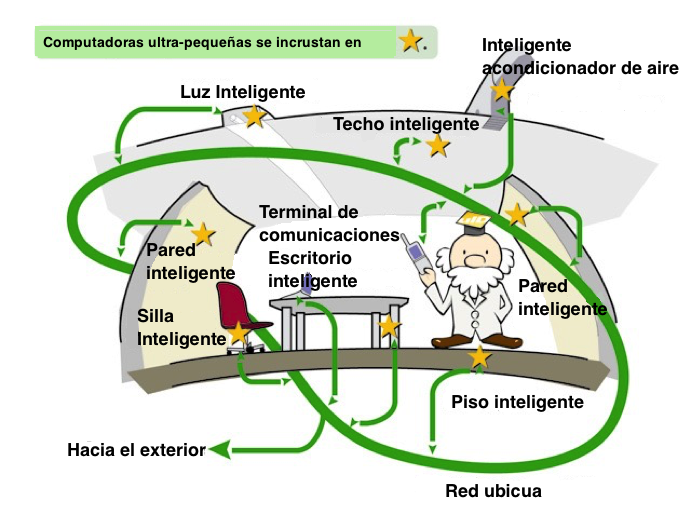
\includegraphics[width=0.8\textwidth]{Figuras/ubicuo.png}
		\rule{35em}{0.5pt}
	\caption[Integración de dispositivos inteligentes en el ambiente]{Integración de dispositivos inteligentes en el ambiente \cite{ubicuo}}
	\label{fig:ubicuo}
\end{figure}

\section{GPS}

\newcommand{\grad}{\hspace{-2mm}$\phantom{a}^{\circ}$}

GPS es la abreviatura de Global Positioning System ó Sistema de Posicionamiento Global en español. Es un sistema de radionavegación basado en satélites desarrollado y controlado por el Departamento de Defensa de Estados Unidos de América que permite a cualquier usuario saber su localización, velocidad y altura, las 24 horas del día, bajo cualquier condición atmosférica y en cualquier punto del globo terrestre. 

Después de la segunda guerra mundial, el Departamento de Defensa de Estados Unidos de América se empeñó en encontrar una solución para el problema del posicionamiento preciso y absoluto. Pasaron varios proyectos y experiencias durante los siguientes 25 años, incluyendo Loran, Transit, etc. Todos permitían determinar la posición pero eran limitados en precisión o funcionalidad. En el comienzo de la década de 70, un nuevo proyecto fue propuesto, el GPS. 

El GPS tiene tres componentes: el espacial, el de control y el de usuario.

El componente espacial está constituido por una constelación de 24 satélites en órbita terrestre aproximadamente a 20200 km, distribuidos en 6 planos orbitales. Estos planos están separados entre sí por aproximadamente 60\grad  en longitud y tienen inclinaciones próximas a los 55\grad  en relación al plano ecuatorial terrestre. Fue concebido de manera que existan como mínimo 4 satélites visibles por encima del horizonte en cualquier punto de la superficie y en cualquier altura.

El componente de control está constituido por 5 estaciones de rastreo distribuidas a lo largo del globo y una estación de control principal (MCS- Master Control Station). Este componente rastrea los satélites, actualiza sus posiciones orbitales y calibra y sincroniza sus relojes. Otra función importante es determinar las órbitas de cada satélite y prever su trayectoria durante las 24 horas siguientes. Esta información es enviada a cada satélite para después ser transmitida por este, informando al receptor local donde es posible encontrar el satélite. 

El componente del usuario incluye todos aquellos que usan un receptor GPS para recibir y convertir la señal GPS en posición, velocidad y tiempo. Incluye además todos los elementos necesarios en este proceso, como las antenas y el software de procesamiento. 

\subsection{Funcionamiento GPS}

Los fundamentos básicos del GPS se basan en la determinación de la distancia entre un punto: el receptor, a otros de referencia: los satélites. Sabiendo la distancia que nos separa de 3 puntos podemos determinar nuestra posición relativa a esos mismos 3 puntos a través de la intersección de 3 circunferencias cuyos radios son las distancias medidas entre el receptor y los satélites. En la realidad, son necesarios como mínimo 4 satélites para determinar nuestra posición correctamente. 

Cada satélite transmite una señal que es recibida por el receptor, éste, por su parte mide el tiempo que las señales tardan a llegar hasta él. Multiplicando el tiempo medido por la velocidad de la señal (la velocidad de la luz), obtenemos la distancia receptor-satélite, (Distancia = Velocidad X Tiempo).

Sin embargo el posicionamiento satelital no es así de simple. Obtener la medición precisa de la distancia no es tarea fácil.

La distancia puede ser determinada a través de los códigos modulados en la onda enviada por el satélite  (códigos C/A y P), o por el análisis de la onda portadora. Estos códigos son complicados. El receptor fue preparado de modo que solamente descifre esos códigos y ninguno más, de este modo él está inmune a interferencias generadas por fuentes naturales o intencionales. Esta es una de las razones para la complejidad de los códigos.  \cite{GPS}
\section{ILS (Indoor Location Systems) Sistemas de Localización en Interiores}

La problemática de la localización en interiores ha sido objeto de un intenso estudio e investigación durante los últimos años. Hasta ahora, ninguna de las soluciones propuestas ha conseguido el éxito que han alcanzado los sistemas de localización y navegación análogos empleados en exteriores, sobre todo el popular GPS. Las razones de este cierto fracaso han sido tanto técnicas como sobre todo económicas: técnicas porque la localización en interiores plantea retos tecnológicos muy superiores a los de la localización en espacios abiertos y económicas porque la mayor parte de los sistemas propuestos utilizan gran cantidad de infraestructura fija (sensores, puntos de control, estaciones base, etc.), lo que hace aumentar mucho el costo.

\subsection{Clasificación de los sistemas ILS}

Por una parte podemos distinguir los sistemas \textbf{basados en tags o etiquetas}, en los cuales el equipo sólo es capaz de detectar y por lo tanto localizar, a aquellos elementos que porten un dispositivo conocido como tag, y por consiguiente al elemento etiquetado.

Por el contrario, los que no precisan de tags son sistemas que sí que son capaces de reconocer y detectar al elemento a seguir.

La ventaja de esta clase de sistemas es que permiten la localización y seguimiento de cualquier elemento, por lo que son de aplicación universal y además son mucho más seguros. No obstante, sus prestaciones son todavía muy limitadas y no son eficaces, excepto en ambientes muy controlados.

Además, están los basados en la \textbf{detección de presencia por un sensor} localizado y de ubicación fija y conocida, llamado punto de control. Una vez detectado el elemento e identificado, la localización del mismo queda acotada a las proximidades del sensor que lo ha identificado. Por consiguiente, la localización se basa en los criterios de presencia y proximidad, dependiendo la precisión del sistema del número de puntos de control desplegados.

También están los sistemas basados en el \textbf{cálculo efectivo de la posición del elemento mediante técnicas de triangulación}, conociendo además otros parámetros como la medida del retardo de propagación o la fuerza de la señal recibida, la ventaja de esta clase de sistemas radica en que alcanzan una gran precisión (en algunos casos del orden de centímetros), y el principal inconveniente se encuentra en el alto costo de la infraestructura a instalar y la complejidad tecnológica.

Por último, citar los equipos basados en el \textbf{análisis del escenario}, que son de mayor complejidad computacional, tratándose de sistemas que analizan determinadas propiedades del escenario en el que se pretende ubicar el elemento para inferir de ellas la posición del mismo. \cite{ILS}

\subsection{Distintas soluciones técnicas}

\subsubsection{Identificación por radiofrecuencia}

Como su nombre indica, son propiamente sistemas de identificación, no de localización, aunque también pueden utilizarse para esta función. Aunque existen multitud de criterios para clasificar los sistemas de RFID, se distinguen dos clases fundamentales en función del tipo de tags que se empleen: pasivos (sin batería) o activos (con batería). Otros criterios de clasificación habituales son la frecuencia de trabajo, si los tags son de sólo lectura o de lectura y escritura, etc. 

Aquí simplemente vamos a presentar las principales características de los tags pasivos y activos. 

Un tag pasivo consiste en una unidad de procesamiento, un transmisor de RF (radiofrecuencia)
y una antena, la cual actúa tanto para la transmisión de la información contenida en el tag (un código de identificación
numérico) como para la alimentación del tag a través de un bucle de inducción a partir de la emisión electromagnética del lector. Cuando el tag cae bajo el radio de acción del lector, el cual emite una señal electromagnética a una determinada frecuencia, el tag carga su batería y transmite su número de identificación, normalmente a una frecuencia distinta. Las principales ventajas de esta clase de tags son su bajo coste, pequeño tamaño y gran duración. En contrapartida el alcance es muy reducido, en torno a un metro en el mejor de los casos, aunque desde hace tiempo se lleva anunciando la salida al mercado de tags pasivos en la banda de UHF (868 MHz en Europa) con alcances de 10 m ó más, pero éstos no acaban de aparecer. La localización se basa en el criterio de proximidad, y la precisión depende del número de puntos de control instalados y la correcta elección de los emplazamientos (por ejemplo, en los puntos de paso forzoso, como en las puertas). En esta clase de sistemas, el coste más elevado por unidad es el de los lectores, aunque en términos globales entre el 50 y el 70% de la inversión total corresponde a los tags. 

Por otra parte están los tags activos, que se caracterizan por disponer de una batería propia que les proporciona la energía suficiente para radiar su código de identificación con mucha mayor potencia que en el caso de los tags pasivos. En consecuencia, el alcance resulta mucho mayor (en torno a los 30 m). Como contrapartida, el coste de los tags activos es mucho mayor, así como su tamaño. El ciclo de vida del tag es el de la batería, que se sitúa alrededor de los 5 años, aunque esto depende de lo intensivo que sea su uso. Los tags activos son apropiados tanto para la implementación de sistemas ILS basados en proximidad (puntos de control), como para sistemas que hagan uso de técnicas de triangulación. 

\subsubsection{Infrarrojos}

Fue la primera tecnología empleada para el desarrollo de sistemas de localización en interiores. Se utilizan tags que emiten radiación infrarroja en modo difuso, es decir, de forma radial, no en modo punto a punto como es habitual en los sistemas IR empleados en comunicaciones. Se trata de un sistema de detección más que de localización, ya que la posición del elemento etiquetado con el tag IR se infiere de la posición fija y conocida de los sensores que detectan al tag. 

La principal limitación de esta alternativa tecnológica es que la radiación infrarroja no atraviesa las paredes, por lo que hay que instalar sensores en cada una de las habitaciones. Además, debido a que la emisión es directiva por el efecto pantalla del cuerpo del portador del tag, es conveniente instalar más de un sensor por localización para asegurar que la detección se produzca correctamente, lo cual hace aumentar mucho el coste. No obstante, con este sistema se obtiene la gran ventaja de conseguir evitar interferencias y falsas detecciones de otros sensores, como sucede en RF. 

\subsubsection{Pinpoint 3D-ID de RF technologies}

PinPoint es un sistema que se basa en estaciones base y tags activos de RFID propietarios de tecnología L3RF (Low range, Long life, Low cost), y requiere el despliegue de una red ad hoc (única para este propósito). 

Los tags se activan al recibir desde una estación base o un controlador de celda (que controla hasta un máximo de 16 antenas), una señal de radio a la frecuencia de 2,4 GHz y responden a intervalos definidos, a la frecuencia de 5,8 GHz con señales que incluyen información de identificación del tag. Observando el retardo de la respuesta del tag en cada estación base o antena, el controlador de celda es capaz de calcular la posición del tag. 

El mayor inconveniente es que cada antena del sistema tiene un área de cobertura muy limitada, las antenas son muy directivas, por lo que es necesario un gran despliegue de infraestructura para cubrir un área, siendo por tanto una solución muy costosa más orientada a naves industriales y almacenes de gran tamaño que a edificios con numerosos tabiques y habitaciones. 

\subsubsection{Radar}

Sistema presentado por Microsoft en marzo del 2000, que hace uso de la tecnología IEEE 802.11. Se basa en las mediciones que las estaciones base de una red WLAN (Wireless LAN) hacen de la potencia y de la relación señal a ruido de las emisiones transmitidas por los dispositivos inalámbricos que se conectan a la red. Una serie de algoritmos permiten estimar la localización de un elemento con una precisión de 3 a 4 m en el 50\% de las ocasiones. Microsoft ha desarrollado dos versiones de la herramienta, una empleando análisis del escenario y otra que emplea triangulación por distancias para el cálculo de la posición. 

La ventaja de este sistema es que requiere, si lo comparamos con otros sistemas, relativamente poca infraestructura. También es interesante que se pueda apoyar sobre redes WLAN ya instaladas para otros propósitos. Como desventajas hay que señalar que sólo pueden ser localizados elementos con capacidad de conexión WLAN y que la aplicación del sistema en edificios con varias plantas, genera problemas de difícil solución debido a que las ondas de radio también pueden atravesar suelos y techos. Así pues, si las señales de un mismo tag son captadas por estaciones base instaladas en plantas distintas, y en función de la potencia con que se reciban, el sistema puede llegar a ubicar al tag en un piso que no le corresponde. Hay que señalar, por otra parte, que las tarjetas WLAN no son baratas y tienen importantes consumos de energía, por lo que difícilmente pueden acomodarse a tags de reducido peso y tamaño. 

\subsubsection{Ultrasonidos}

Se trata de soluciones que están también basadas en tags o etiquetas para los elementos a controlar, pero en este caso estos tags emiten o reciben ultrasonidos. El sistema más representativo es el Bat de AT\&T Laboratories. Los tags cuentan con un transceptor radio (banda de 433 MHz), una lógica de control que contiene un identificador único de 48 bits y un emisor de ultrasonidos. La infraestructura se compone de sensores de ultrasonidos, estaciones base de RF y un sistema central de gestión, formando los sensores o receptores una malla en puntos conocidos del techo. Una estación base transmite periódicamente un mensaje que contiene el identificador del tag que desea activar y al recibir el mensaje con su identidad, el tag aludido se despierta y emite un pulso de muy corta duración. Además, se resetea el reloj de los sensores del área de influencia, los cuales comienzan a contar el tiempo que transcurre hasta que reciben la señal del tag Bat. A partir de este retardo y de la velocidad de propagación del sonido en el aire, se calcula de forma inmediata la distancia al sensor. Cabe destacar que con las distancias del tag a varios sensores (mínimo tres), puede conocerse la posición del tag en 3 dimensiones. Este sistema es capaz de detectar la posición de los tags con un error máximo de 3 cm en un 95\% de las medidas. Cada estación base puede activar simultáneamente un número máximo de 3 tags, con una frecuencia de refresco de 50 veces por segundo. El tiempo de vida de la batería del tag es de 15 meses. El sistema Bat no se comercializa en la actualidad debido al alto coste de la infraestructura, que se espera poder reducir en posteriores versiones del sistema. Otro de los retos que pretenden acometer los investigadores de AT\&T es la sustitución de las comunicaciones RF entre estaciones base y tags por IR para evitar la complejidad del trabajo multifrecuencia en estaciones base próximas. En cualquier caso, se trata de una tecnología poco madura y bastante elevada en precio, encontrándose todavía lejos de ser comercializada. 

\subsubsection{Visión Artificial}

Estos sistemas hacen uso de la información recogida por cámaras y utilizan técnicas de procesamiento de imágenes para la identificación y seguimiento de objetos. Estos sistemas de visión empleados en identificación y localización pueden trabajar tanto con marcadores visuales (tags) como sin ellos. 

\subsubsection{Zigbee}

Iniciado por Philips, Honeywell, Invensys y seguido por Motorota, Mitsubishi y hasta 25 empresas para crear un sistema estándar de comunicaciones inalámbrico y bidireccional, para usarlo dentro de dispositivos de domótica, automatización de edificios (inmótica), control industrial, periféricos de PC, sensores médicos e identificación y localización. La idea de ponerle el nombre ZigBee vino de una colmena de abejas pululando alrededor de su panal y comunicándose entre ellas.
Los miembros de esta alianza justifican el desarrollo de este estándar para cubrir el vacío que se produce por debajo del Bluetooth. Puede transmitir con un simple protocolo de 20 KB/s trabajando a una frecuencia de 2,4 GHz (banda libre ISM) u 868 MHz (Europa) o 915 MHz (EEUU), con bajo consumo (“transceiver” ZigBee dormido la mayor parte del tiempo), rangos entre 10 y 75 metros y soporte de hasta 255 nodos. 

\subsubsection{Campo Magnético}

Los sistemas de localización basados en el campo magnético de la tierra pueden ser agrupados principalmente en dos categorías, aquellos que requieren de una fase pasiva más extensa y detallada, refiriéndose a una recolección de información meticulosa dividiendo el área en superficies pequeñas de igual tamaño y obtener para cada una de esas pequeñas superficies su lectura del campo magnético \cite{usoCampoMagnetico}, como lo podemos visualizar en la Figura \ref{fig:ejPasiva}.

\begin{figure}[htbp]
	\centering
		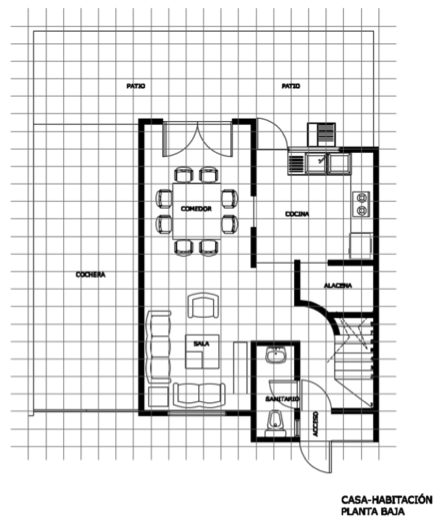
\includegraphics{Figuras/ejPasiva.png}
		\rule{35em}{0.5pt}
	\caption[División de una casa habitación para la recolección de información en la fase pasiva]{Ejemplo de división de una casa habitación para la recolección de información en la fase pasiva}
	\label{fig:ejPasiva}
\end{figure}

Por otro lado, se tiene el enfoque siguiendo al líder (follow the leader), en el cual la fase pasiva es mucho más sencilla, ya que solamente consta de recolectar información dentro de la habitación generando un perímetro o recorrido predefinido que en la fase activa puede ser reconocido y así obtener la localización, enfoque representado en la Figura \ref{fig:ejSigLider}.

 \begin{figure}[htbp]
	\centering
		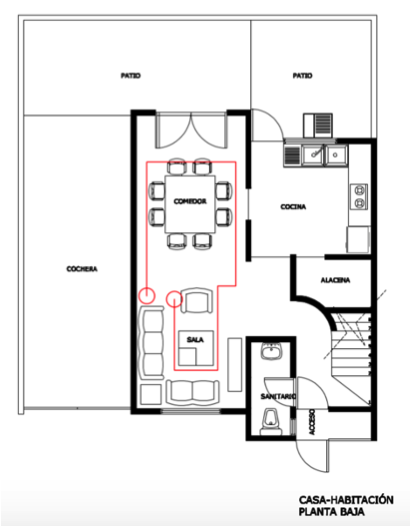
\includegraphics{Figuras/ejSigLider.png}
		\rule{35em}{0.5pt}
	\caption[Perímetro requerido en el enfoque siguiendo al líder  para reconocer una habitación]{Ejemplo de perímetro requerido en el enfoque siguiendo al líder  para reconocer una habitación}
	\label{fig:ejSigLider}
\end{figure}
\section{Sistema Operativo Móvil Android}

Android es un sistema operativo y una plataforma software, basado en Linux, que junto con aplicaciones middleware está enfocado para ser utilizado en dispositivos móviles como teléfonos inteligentes, tabletas, google TV y otros dispositivos. Android permite programar en un entorno de trabajo (framework) de Java, lo que nos asegura que podrán ser ejecutadas en cualquier tipo de CPU, tanto presente como futuro. Aplicaciones sobre una máquina virtual Dalvik (una variación de la máquina de Java con compilación en tiempo de ejecución creada por Google optimizada para dispositivos móviles). Además, lo que le diferencia de otros sistemas operativos, es que cualquier persona que sepa programar puede crear nuevas aplicaciones, widgets o incluso, modificar el propio sistema operativo, dado que Android es de código libre. \cite{Android}

\begin{figure}[htbp]
	\centering
		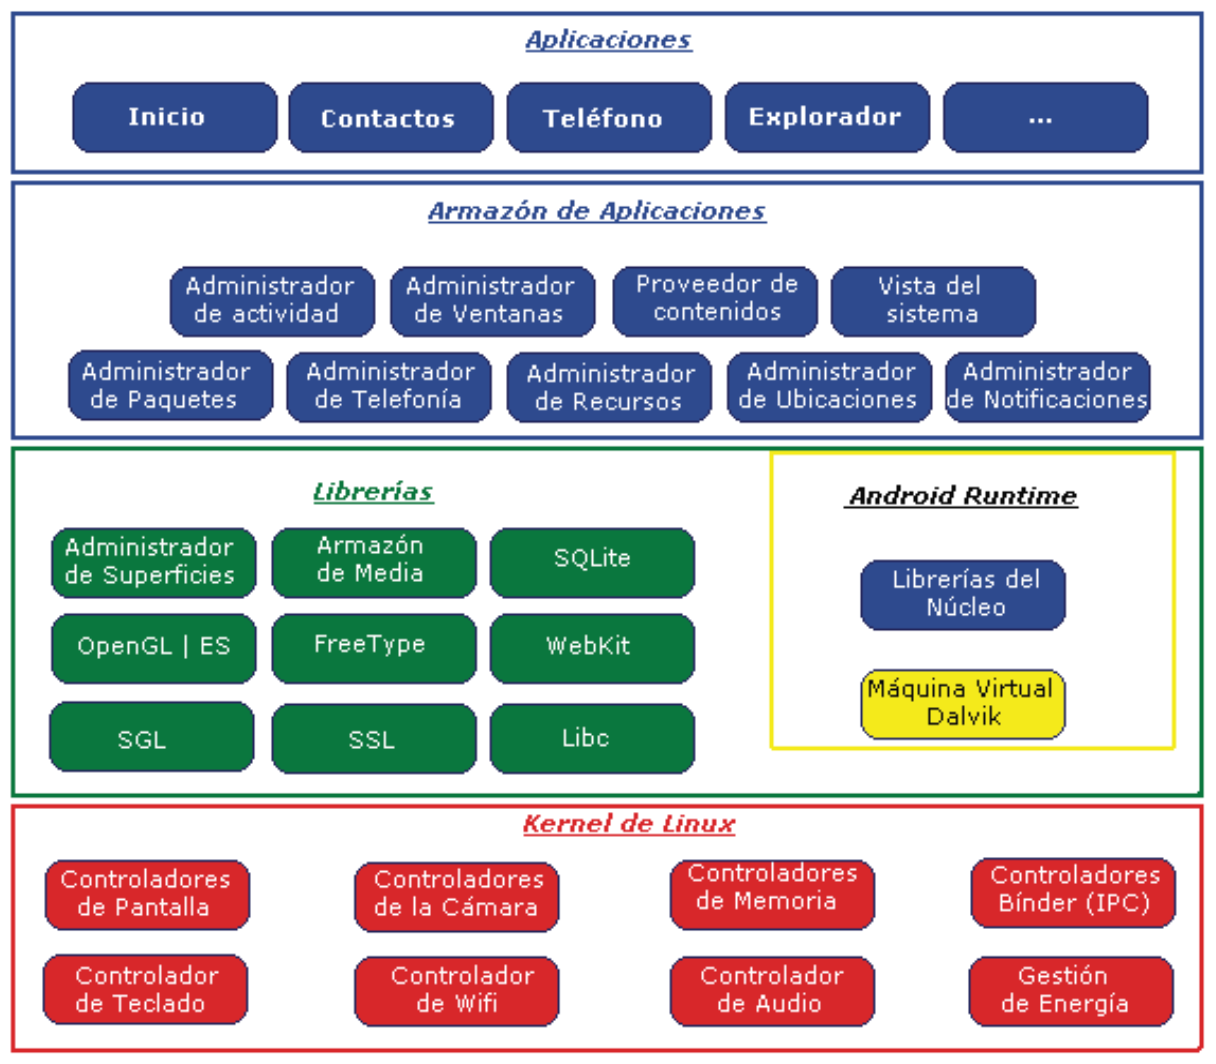
\includegraphics[width=1\textwidth]{Figuras/capasAndroid.png}
		\rule{30em}{0.5pt}
	\caption[Sistema de capas de Android]{Sistema de capas de Android}
	\label{fig:capasAndroid}
\end{figure}

En la Figura \ref{fig:capasAndroid} se distinguen claramente cada una de las capas: la que forma parte del propio Kernel de Linux, donde Android puede acceder a diferentes controladores, las librerías creadas para el desarrollo de aplicaciones Android, la siguiente capa que organiza los diferentes administradores de recursos, y por último, la capa de las aplicaciones a las que tiene acceso.

\begin{itemize}
	\item \textbf{Arquitectura basada en componentes}
	\begin{itemize}
		\item El diseño de la interfaz de usuario se hace en xml, lo que permite que una misma aplicación se ejecute en un dispositivo móvil de pantalla reducida o en un TV.
	\end{itemize}
	\item \textbf{Filosofía de dispositivo siempre conectado a Internet}
	\begin{itemize}
		\item Servicios incorporados basados en Web.
		\item Localización basada tanta en GPS como en redes, bases de datos con SQL, navegadora, multimedia.
	\end{itemize}
	\item \textbf{Aceptable nivel de seguridad}
	\begin{itemize}
		\item Los programas se encuentran aislados unos de otros gracias al concepto de ejecución dentro de una caja que hereda de Linux.
		\item Cada aplicación dispone de una serie de permisos que limitan su rango de actuación (servicios de localización, acceso a Internet, etc.)
	\end{itemize}
	\item \textbf{Calidad de gráficos y sonido}
	\begin{itemize}
		\item Gráficos en 3 dimensiones basados en OpenGL.
		\item Gráficos vectoriales suavizados.
		\item Animaciones inspiradas en Flash.
		\item Incorpora codecs estándar más comunes de audio y vídeo, incluyendo H.264 (AVC), MP3, AAC, etc.
	\end{itemize}
\end{itemize}

\subsection{Características de Android}

\begin{itemize}
	\item \textbf{Acceso a Hardware, incluyendo Cámara, GPS y Sensores: }Android incluye API’s que permite simplificar el desarrollo sin importar el hardware sobre el que se está trabajando. Esto asegura que no necesitamos crear implementaciones específicas para distintos dispositivos, así que podemos crear aplicaciones que deben trabajar según lo esperado en cualquier dispositivo que tenga una versión compatible de Android.
	\item \textbf{Transferencia de Datos con Wi-Fi, BlueTooth y NFC: } Android ofrece soporte muy completo para transferir datos entre dispositivos, incluyendo Bluetooth, Wi-Fi y Android Beam. Estas tecnologías permiten compartir datos entre dispositivos, dependiendo del hardware disponible en el dispositivo utilizado.
	\item \textbf{Mapas y Geolocalización: }El manejo de mapas embebido con el que cuenta Android permite crear aplicaciones que de manera programática pueden manipular los mapas de Google Maps. Además, la integración de un GPS y los servicios de localización de Google para determinar la ubicación actual del dispositivo, permite combinar posicionamiento con mapas.
	\item \textbf{Servicios en Segundo Plano (Background Services): }Android soporta aplicaciones y servicios diseñados para ser ejecutados en segundo plano, mientras nuestra aplicación no está activa, debido a que solamente una aplicación puede estar visible a la vez. 
	\item \textbf{Base de Datos SQLite: }El almacenamiento y la recuperación de información de manera rápida y eficiente es básica para dispositivos con capacidad limitada. Android utiliza SQLite para cumplir con este objetivo. Las aplicaciones móviles pueden aprovechar esta base de datos relacional para almacenar y recuperar información de manera segura y eficiente.
	\item \textbf{Compartición de Datos y Comunicación entre Aplicaciones: }Android incluye técnicas para compartir información entre las distintas aplicaciones, tales como: Intents y Content Providers.
	\item \textbf{ Soporte para gráficos 2D y 3D: }Android provee librerías gráficas para dibujos 2D y 3D con OpenGL. Además, Android provee soporte para imágenes, video, audio, incluyendo video en formato mpeg4.
	\item \textbf{Optimización de Memoria y Administración de Procesos: }Android utiliza su propia maquina virtual para la administración de la memoria. Android asegura que una aplicación responda en un tiempo determinado, de lo contrario la detiene y la puede eliminar en caso de ser necesario, con el objetivo de liberar recursos. De esta manera Android controla el ciclo de vida de las aplicaciones en un ambiente enfocado en hacer más eficiente el uso de memoria de los dispositivos. \cite{presentacionAndroid}
\end{itemize}
